% !TeX spellcheck = en_US

% Master Project Paper: Tangible Horror
% Alexandra R. Müller & Leonie F. E. Ferdinand
% Hochschule RheinMain – University of Applied Sciences and Arts (HSRM)
%
% Build with ./build.sh (pdflatex + bibtex + 2x pdflatex).
%
% Document layout:
%   chapters/   one file per top-level unit of the paper; each file carries
%               only the \section heading and \input lines
%   sections/   the actual text, one subfolder per chapter
% To add content, create a file under sections/<chapter>/ and add a matching
% \input line to the chapter file.

\documentclass[sigconf,nonacm]{acmart}

% Page numbers on (useful while drafting)
\settopmatter{printfolios=true}

\usepackage{booktabs}
% placeins' [section] option redefines \section, which acmart rejects.
% Load it plain and use \FloatBarrier explicitly where a section must hold its floats.
\usepackage{placeins}
\usepackage{subcaption}   % (a)/(b) labels inside a multi-panel figure
\usepackage{adjustbox}    % provides \clipbox, used by \coverimg below

% Float placement. LaTeX reserves a lot of each page for text by default, which
% pushes big figures onto later pages; these give figures more room at the top.
% The dbl... versions apply to full-width figure* floats in two-column mode, and
% dblfloatfix stops LaTeX deferring such a float further than it needs to.
\usepackage{dblfloatfix}
\renewcommand{\topfraction}{0.9}
\renewcommand{\dbltopfraction}{0.9}
\renewcommand{\textfraction}{0.07}
\renewcommand{\floatpagefraction}{0.75}
\renewcommand{\dblfloatpagefraction}{0.75}
\setcounter{topnumber}{3}
\setcounter{dbltopnumber}{2}
\setcounter{totalnumber}{4}

% Look for images here, so a \coverimg only needs the bare file name.
\graphicspath{{figures/}{../study-photos/}{../ingame-photos/}}

% --- image helpers --------------------------------------------------------
% Photos out of a phone are portrait and huge. Never give \includegraphics both
% a width and a height without keepaspectratio: that stretches the picture.
% Use one of these two instead.
%
% \figimg{<height>}{<file>}
%   Fits the whole image inside the column width AND the given height. Nothing
%   is stretched or cut off, but a portrait photo leaves white space beside it.
\newcommand{\figimg}[2]{%
  \includegraphics[width=\linewidth,height=#1,keepaspectratio]{#2}}
%
% \coverimg[<bias>][<trim>]{<height>}{<file>}
%   Fills the column at exactly the given height and crops whatever does not
%   fit. The aspect ratio is kept, so nothing is stretched. Use this for panels
%   that must line up in a grid.
%   <bias>  which part survives the automatic crop: 0 = keep the top (or left),
%           0.5 = keep the middle (default), 1 = keep the bottom.
%   <trim>  optional extra crop taken off the source photo BEFORE it is fitted,
%           given as "left bottom right top". Use fractions of \height and
%           \width so it does not depend on the pixel size of the photo, e.g.
%           [0.5][0 {.3\height} 0 0] cuts the bottom third away first.
%   Both options are positional: to pass a trim you must also pass a bias.
\newsavebox{\covbox}
\newlength{\covl}\newlength{\covb}\newlength{\covr}\newlength{\covt}
\NewDocumentCommand{\coverimg}{ O{0.5} O{0 0 0 0} m m }{%
  % adjustbox (not plain graphicx) is what accepts \height/\width in a trim.
  \sbox\covbox{\adjustbox{trim={#2},clip,width=\linewidth}{\includegraphics{#4}}}%
  \ifdim\ht\covbox<#3\relax
    \sbox\covbox{\adjustbox{trim={#2},clip,height=#3}{\includegraphics{#4}}}%
  \fi
  \setlength{\covl}{\wd\covbox}\addtolength{\covl}{-\linewidth}%
  \setlength{\covt}{\ht\covbox}\addtolength{\covt}{-#3}%
  \setlength{\covr}{\covl}\setlength{\covb}{\covt}%
  \setlength{\covl}{#1\covl}\addtolength{\covr}{-\covl}%
  \setlength{\covt}{#1\covt}\addtolength{\covb}{-\covt}%
  % \clipbox does not expand its argument, so build it with \edef first.
  \edef\covargs{\the\covl\space\the\covb\space\the\covr\space\the\covt}%
  \expandafter\clipbox\expandafter{\covargs}{\usebox\covbox}}

% Draft placeholder for figures whose image files do not exist yet.
% To use a real image: comment out the \phold line and uncomment the
% \includegraphics line above it. Remove this macro once all are replaced.
\newcommand{\phold}[2]{%  #1 = box height, #2 = what the panel should show
  \fcolorbox{black!30}{black!5}{%
    \begin{minipage}[c][\dimexpr#1-2\fboxsep-2\fboxrule\relax][c]{\dimexpr\linewidth-2\fboxsep-2\fboxrule\relax}
      \centering\footnotesize\itshape\color{black!60}#2
    \end{minipage}}}

% Draft marker for missing numbers and open decisions.
% Remove all \todoin{...} before submission.
\newcommand{\todoin}[1]{\textcolor{red}{\textbf{[TODO: #1]}}}

\begin{document}

\title[Tangible Horror]{Tangible Horror: Passive Haptic Proxies in a Virtual Reality Horror Experience}

\author{Alexandra R. Müller}
\email{alexandra.mueller\_1@student.hs-rm.de}
\affiliation{%
  \institution{Hochschule RheinMain}
  \city{Wiesbaden}
  \country{Germany}
}

\author{Leonie F. E. Ferdinand}
\email{leoniefranziskaelisabeth.ferdinand@student.hs-rm.de}
\affiliation{%
  \institution{Hochschule RheinMain}
  \city{Wiesbaden}
  \country{Germany}
}

\begin{abstract}
  % !TeX root = ../paper.tex

Touch is the sense that current consumer VR serves worst. A player who reaches for a virtual object and grasps empty air is reminded, at exactly the wrong moment, that none of it is real. We built \emph{Tangible Horror}, a room-scale horror experience for the Meta Quest~3 in which a player wakes up locked inside a cabin and must recover four hidden coins to escape. Each hiding place doubles as a small ordeal: a bowl filled with eyes, a bucket of maggots, a leaking pipe that sprays blood, and cobwebs behind a closet. In the haptic condition, every one of these ordeals has a physical counterpart the player actually touches---rubber balls, gummy worms, water sprayed from a bottle, and synthetic spider webbing---aligned with the virtual scene through spatial anchors and marker-based tracking. In a within-subject study with seven participants (five of whom played both conditions in randomized order), each playthrough was followed by the Igroup Presence Questionnaire (IPQ). The haptic condition scored markedly higher on every IPQ subscale---general presence, spatial presence, involvement, and experienced realism---and every participant who played both versions rated the haptic one higher on all four. Given the small sample, we report these differences descriptively, but their size and consistency are hard to dismiss. We describe the design of the four proxy challenges, the technical setup, and what our results suggest about low-cost passive haptics as a tool for presence in emotionally charged VR.

\end{abstract}

\keywords{virtual reality, passive haptics, presence, immersion, horror, tangible proxies, IPQ}

% Teaser: the full-width strip under title and authors on page 1.
% Three panels, or drop to two by widening them to 0.49\textwidth.
\begin{teaserfigure}
  \begin{minipage}[c]{0.325\textwidth}
    \coverimg{3.0cm}{room.jpeg}
  \end{minipage}\hfill
  \begin{minipage}[c]{0.325\textwidth}
    \coverimg{3.0cm}{bucket-inside.jpeg}
  \end{minipage}\hfill
  \begin{minipage}[c]{0.325\textwidth}
    \coverimg{3.0cm}{room-virtual.png}
  \end{minipage}
  \caption{In \emph{Tangible Horror} the player is locked in a cabin (right) and has to discover four coins from four unpleasant hiding places. In the haptic condition each hiding place has a physical counterpart (left) the player reaches into with bare hands, here a bucket of gummy worms standing in for a bucket of maggots (middle).}
  \Description{Three panels: the study room with proxy stations, the proxy bucket and gummy worms, and the virtual room with all challenges.}
  \label{fig:teaser}
\end{teaserfigure}

\maketitle

% !TeX root = ../paper.tex

\section{Introduction}
\label{sec:introduction}

% !TeX root = ../../paper.tex

Modern VR headsets are particularly effective at stimulating the senses of sight and hearing but they offer no resistance when the player reaches out. This limitation becomes especially apparent in the moments when a VR experience works hardest to create an immersive situation. The player leans in, stretches out a hand, and touches nothing. Force-feedback hardware and haptic suits could close the gap, but they remain expensive, cumbersome, and restrict free movement. Passive haptics skips the hardware. It involves placing real objects at the locations where the virtual objects appear to be, so that the player's hand finds what their eyes expect~\cite{Insko.2001, substitutional-reality}.

The horror genre is built on anticipation: the player knows something unpleasant is coming and has to act anyway. Reaching into a bowl one cannot see into is unsettling on a screen; when the hand sinks into something cold and yielding, the stakes change. Horror also punishes broken illusions, because a scare loses its force the moment a hand swipes through empty air. Presence and fear are coupled in VR: in virtual height exposure the two correlate at $r = .62$~\cite{Gromer.2019}, and adding a physical ledge to a virtual pit raised participants' heart-rate response as well as their reported presence~\cite{Meehan.2002}. If passive haptics changes presence at all, an experience built on disgust and fear should make the difference visible.

\emph{Tangible Horror}, our VR escape scenario for the Meta Quest~3, puts this to the test. The game locks the player in a run-down cabin; to open the lock on the door, they must collect four coins, each hidden inside a small horror challenge that the player has to reach into.
In the haptic condition each challenge is supplemented by a low-cost physical proxy (rubber balls, gummy worms, a water-spraying tube operated by an experimenter, and synthetic Halloween webbing) aligned with its virtual counterpart. In the baseline condition the player plays the identical scene and touches nothing but air. We compared both conditions within participants, in randomised order, using the Igroup Presence Questionnaire (IPQ)~\cite{Schubert.2001} after each playthrough.

This paper makes two contributions. First, we describe the design and implementation of the four proxy challenges, including the practical work that decides whether a proxy illusion holds: calibrating virtual object sizes to their physical stand-ins, anchoring furniture in the tracking space, and tracking hand-held coins with fiducial markers. Second, we report an empirical comparison of the haptic and non-haptic versions of the same experience. Section~\ref{sec:related-work} situates the project in prior work on passive haptics and on presence and emotion in VR. Sections~\ref{sec:apparatus} and~\ref{sec:study} describe the prototype and the study; Sections~\ref{sec:results} and~\ref{sec:discussion} present and discuss the results.


% !TeX root = ../paper.tex

\section{Related Work}
\label{sec:related-work}

% !TeX root = ../../paper.tex

\subsection{Passive Haptics and Proxy Objects}
\label{sec:rw-passive-haptics}

The core observation behind passive haptics predates consumer VR by two decades. Hoffman showed in 1998 that letting participants pick up a real plate while seeing its virtual twin made them rate other virtual objects as more solid and the environment as more realistic~\cite{Hoffman.1998}. Insko's dissertation work made the case more dramatically: participants who felt a low wooden ledge under their feet while standing at a virtual pit showed stronger presence responses than those who only saw the drop~\cite{Insko.2001}. Both studies used proxies that were far simpler than the objects they stood in for, which is what makes the technique attractive---the haptic channel apparently does not demand the fidelity the visual channel does.

How much discrepancy players tolerate is the question Simeone et al.\ addressed with Substitutional Reality~\cite{substitutional-reality}. They systematically mismatched physical objects and their virtual representations---an umbrella standing in for a lightsaber being the canonical example---and derived guidelines for which properties (size, shape, temperature, weight) can drift and which break the illusion. Their participants kept accepting substitutions well past the point of literal resemblance, provided the mismatch did not contradict what the hand felt at first contact. Azmandian et al.\ pushed in the other direction with haptic retargeting, warping the virtual world so that a single physical cube could serve as the proxy for several virtual objects in different locations~\cite{Azmandian.2016}.

Our project sits deliberately at the low-tech end of this spectrum. We use no retargeting and no instrumented props; each virtual object has one fixed physical counterpart chosen for its texture rather than its geometry. What distinguishes our setup from the studies above is the emotional register of the materials. Prior proxy work has mostly paired neutral objects---cubes, plates, furniture. We pair proxies with content designed to disgust, which raises a question the literature leaves open: whether confirming the player's worst tactile expectations amplifies the emotional response, or whether the mundane identity of the proxy (a gummy worm is, after all, candy) undercuts it.

% !TeX root = ../../paper.tex

\subsection{Presence and Emotion in VR}
\label{sec:rw-presence-emotion}

Presence---the sense of being in the virtual place rather than merely looking at it---is the standard yardstick for experiences like ours. Slater's distinction between place illusion and plausibility~\cite{Slater.2009} maps well onto what a haptic proxy is supposed to deliver: touch that confirms vision should strengthen the plausibility of events, not just the sense of location. The most common way to measure presence remains the questionnaire. We use the Igroup Presence Questionnaire (IPQ)~\cite{Schubert.2001}, which separates general presence, spatial presence, involvement, and experienced realism. Questionnaires are a blunt instrument, and their sensitivity varies with the presence dimension being manipulated~\cite{presence-questionnaires}, but for a two-condition comparison of the same experience they remain the pragmatic choice.

A second strand of work examines how VR shapes emotional and physiological responses. Kobayashi et al.\ compared identically furnished real and virtual rooms and found that the VR versions produced higher arousal even though the real rooms were judged more pleasant~\cite{Kobayashi.2025}---VR is not emotionally neutral ground to begin with. Khundrakpam et al.\ used VR exercises to elicit distinct stress responses in a controlled way~\cite{Khundrakpam.2025}, Marocco et al.\ showed that arousal in VR is not simply negative, since physiologically activating nature scenes were experienced as restorative~\cite{Marocco.2025}, and Zhang et al.\ demonstrated that even the color of a virtual workspace shifts self-reported and physiological emotion~\cite{Zhang.2025}. For horror specifically, Lin studied a commercial zombie game and catalogued which elements of a VR horror experience players report as frightening and how they cope, including next-day effects~\cite{Lin.2017}.

Taken together, this work establishes that VR reliably provokes strong emotional responses and that presence and emotion are entangled. What it does not tell us is how a deliberately unpleasant tactile stimulus feeds into that loop. That gap is where this project sits: we hold the virtual content constant and vary only whether the player's hands find the expected horror or nothing at all.


% !TeX root = ../paper.tex

\section{Apparatus}
\label{sec:apparatus}

The player starts inside a dimly lit wooden cabin. A lock with four coin-shaped slots bars the front door; the way out is to find four golden coins hidden around the room and insert them into the lock. Dark ambient music and the cramped, cluttered interior set the tone before anything threatens the player.

Each coin hides inside one of four challenges, described in Section~\ref{sec:apparatus-challenges}, so the search forces the player to interact with every station in the room. The game has no time limit and no fail state; players can take as long as they want, and nothing punishes hesitation. The discomfort lies in what the player has to touch to get each coin. Once the fourth coin clicks into place, the lock opens and a win screen ends the session. We chose this flow for the study because it guarantees that each participant encounters all four haptic (or non-haptic) interactions in a single playthrough, while leaving the order of the challenges up to the player.

A game manager script drives this loop. The same scene runs in both study conditions; the conditions differ in whether the physical proxies lie in the tracking space at the positions of their virtual counterparts.

% !TeX root = ../../paper.tex

\subsection{The Four Challenges}
\label{sec:apparatus-challenges}

Each challenge pairs a virtual horror object with an everyday physical proxy chosen to match its expected texture. The proxies cost a few euros each; none of them is instrumented.

\paragraph{Bowl of eyes.} A rusted bowl on a wooden table is filled with realistic looking eyeballs. The player has to dig through them to find the coin at the bottom of the bowl. The physical proxy is a real metal bowl filled with rubber balls whose size matches the virtual eyes exactly; the virtual bowl is scaled at runtime to the measured dimensions of the physical one, so the rim is where the hand expects it.

\paragraph{Bucket of maggots.} A wooden bucket teems with writhing maggots, again with a coin buried underneath. The proxy is a bucket of gummy worms. Their damp, slightly sticky surface and the way a handful gives under pressure come close to what the visuals promise, at least closer than any dry material we tried.

\paragraph{Bloody pipe.} A pipe assembly bursts when the player pulls out the coin and sprays blood at them, driven by a particle system. The haptic counterpart is deliberately low-tech, in the tradition of Wizard-of-Oz setups: a researcher standing outside the play area sprays a fine mist of water from a bottle through a plastic tube aligned with the virtual pipe, timed to the burst. The spray lasts around five seconds and then stops together with the particle effect.

\paragraph{Cobwebs behind the closet.} The last coin hides behind a closet, in a mass of spider webs the player has to reach into. The proxy is synthetic Halloween spider webbing stretched behind an upright table. The material clings to skin and stretches when the hand pulls back---a sensation that is hard to fake with anything else and unpleasant even when one knows exactly what it is. The coin itself is hanging on a thin string, so the player feels the sensation of ripping it free when they attempt to remove it.

The set covers a deliberate range of contact types: immersing the whole hand (eyes, worms), a sudden stimulus arriving on the body (spray), and a clinging texture the player has to pull free from (webs). It also varies who controls the moment of contact---the player in three challenges, the experimenter in one.

% !TeX root = ../../paper.tex

\subsection{Implementation and Alignment}
\label{sec:apparatus-implementation}

The prototype runs standalone on a Meta Quest~3 and is built in Unity~6 with the Universal Render Pipeline, using the Meta XR SDK via OpenXR. The cabin interior, props, and creatures are assembled from asset store packs; custom scripts handle everything specific to the study.

Getting a proxy illusion to hold comes down to alignment, and we use two mechanisms depending on whether an object moves. Static furniture and the proxy stations are aligned by hand during setup: the experimenter places the physical bowl, bucket, pipe outlet, and webbing in the room, adjusts the corresponding virtual objects to match, and pins the result with the Quest's spatial anchors so the calibration survives headset restarts and short tracking losses. A dedicated authoring mode supports this step, and a world-lock component keeps each virtual object fixed to its anchored real-world pose at runtime.

The coins are the one thing the player carries around, so a static anchor is not enough. Physical coin props are tracked optically through the headset's passthrough cameras using AprilTag fiducial markers, with a One-Euro filter smoothing the raw poses. The virtual coin follows its physical twin, which lets a participant fish a coin out of the maggot bucket, hold onto it, and slot it into the door lock, with the virtual and physical coin staying in register throughout.

Scale mismatches are handled at the source: a sizing component scales each virtual object so that its rendered dimensions match the measured dimensions of its physical proxy in centimeters, either uniformly or per axis. This mattered more than expected---a virtual bowl a few centimeters wider than the real one is enough for the player's fingers to visibly clip through the rim on approach.


% !TeX root = ../paper.tex

\section{Study}
\label{sec:study}

% !TeX root = ../../paper.tex

\subsection{Study Design}
\label{sec:study-design}

We compared two conditions in a within-subject design. In the \emph{haptic} condition, all four physical proxies were in place and aligned with their virtual counterparts; in the \emph{baseline} condition, participants played the identical scene with no physical objects in the play area. Participants played both conditions in a single session, completing the full cabin escape each time. The order of conditions was randomized per participant to counter order effects; of the five participants who completed both conditions, three started with the haptic version and two with the baseline. Two further participants played only the haptic version (see Section~\ref{sec:study-participants}).

The condition comparison is deliberately coarse: proxies are either all present or all absent. A per-challenge manipulation would have been more informative about which proxy carries the effect, but at the cost of a much larger design; with a single playthrough per condition we judged the all-or-nothing contrast to be the honest scope for a project of this size.

% !TeX root = ../../paper.tex

\subsection{Participants}
\label{sec:study-participants}

\todoin{N} participants took part in the study (\todoin{age range, mean age, gender distribution; prior VR experience if collected}). Participants were recruited \todoin{how---fellow students, word of mouth?} and took part voluntarily without compensation. \todoin{Adjust if there was compensation, and add anything participants were told or asked beforehand, e.g.\ warnings about horror content, allergies regarding the gummy worms, consent form details.}

% !TeX root = ../../paper.tex

\subsection{Procedure}
\label{sec:study-procedure}

Sessions took place in a work room at Hochschule RheinMain that was prepared as the play area, with the proxy stations set up and calibrated before participants arrived. After a short briefing on the headset, the controls, and the horror content---participants knew the genre but not the individual challenges---each participant put on the Quest~3 and played their first condition until they escaped the cabin. They then took the headset off and filled in the IPQ. The same steps were repeated for the second condition, followed by the second IPQ. \todoin{Add: informed consent step, whether hands were disinfected / gummi worms handled hygienically, whether participants could abort, and the typical session length.}

Between conditions the experimenters added or removed the physical proxies, depending on the assigned order. One researcher operated the water spray for the pipe challenge in the haptic condition, watching the mirrored headset view to time the spray to the virtual burst. \todoin{Confirm: was the view mirrored/cast to a laptop?}

% !TeX root = ../../paper.tex

\subsection{Measures}
\label{sec:study-measures}

Presence was measured with the Igroup Presence Questionnaire (IPQ)~\cite{Schubert.2001}, completed once after each condition. The IPQ consists of 14 items on 7-point scales and yields a general presence item (``the sense of being there'') plus three subscales: spatial presence, involvement, and experienced realism. We chose the IPQ over alternatives because its subscales map onto the aspects a haptic manipulation should plausibly move---experienced realism above all---and because it is short enough to administer twice in one session without wearing participants down~\cite{presence-questionnaires}.

Our exposé additionally planned the Self-Assessment Manikin and heart rate variability as emotional and physiological measures. Both were dropped during the project to keep the study sessions manageable; we return to this reduction in scope in Section~\ref{sec:discussion-limitations}. \todoin{Rephrase or drop this admission if you would rather not flag it here.}


% !TeX root = ../paper.tex

\FloatBarrier
\section{Results}
\label{sec:results}

% !TeX root = ../../paper.tex

Questionnaire responses were scored following the anchors of the administered form: all items use 7-point scales, and items~1 (``How aware were you of the real world\ldots''), 11 (``I still paid attention to the real environment'') and 13 (``I felt like I was just perceiving pictures'') were reverse-coded so that higher values always indicate more presence. Item~6 needed no recoding, as its response anchors already run from ``did not feel present'' to ``felt present''. Subscale scores are item means: general presence (item~8), spatial presence (items 3, 6, 9, 10, 13), involvement (items 1, 7, 11, 14), and experienced realism (items 2, 4, 5, 12), following the IPQ structure~\cite{Schubert.2001}.

Descriptive statistics cover all twelve playthroughs (haptic $n=7$, baseline $n=5$); the paired analysis uses the five participants who completed both conditions. Table~\ref{tab:ipq-results} summarizes both.

\begin{table}[t]
  \caption{IPQ subscale scores (1--7), reported as $M$ ($SD$) over all playthroughs; $\Delta$, $t$, and $d_z$ from the five complete pairs.}
  \label{tab:ipq-results}
  \small
  \setlength{\tabcolsep}{4.5pt}
  \begin{tabular}{lccccc}
    \toprule
    Subscale & Haptic & Baseline & $\Delta$ & $t(4)$, $p$ & $d_z$ \\
    \midrule
    General presence     & 5.71 (0.49) & 2.40 (0.55) & $+3.20$ & 6.53, .003 & 2.92 \\
    Spatial presence     & 6.09 (0.70) & 2.96 (0.50) & $+3.12$ & 6.87, .002 & 3.07 \\
    Involvement          & 5.04 (0.88) & 2.15 (0.63) & $+2.65$ & 7.39, .002 & 3.30 \\
    Experienced realism  & 4.36 (1.17) & 2.25 (0.47) & $+2.05$ & 5.05, .007 & 2.26 \\
    \bottomrule
  \end{tabular}
\end{table}

\begin{figure}[t]
  \centering
  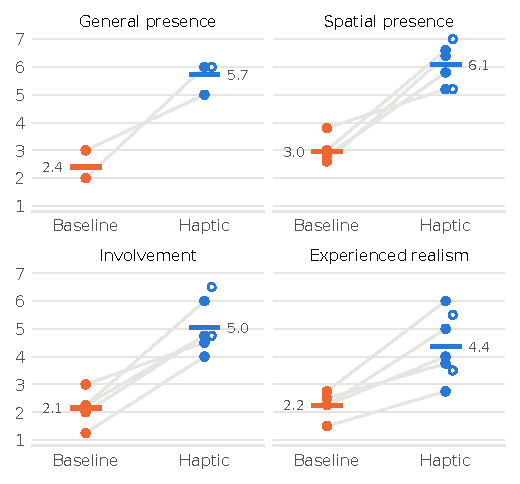
\includegraphics[width=\columnwidth]{figures/ipq_subscales}
  \caption{IPQ subscale scores per condition. Gray lines connect the two playthroughs of the same participant ($n=5$); open circles are the two participants who played only the haptic condition; horizontal ticks mark condition means over all playthroughs.}
  \Description{Four slope panels, one per IPQ subscale. In each panel every connecting line rises steeply from the baseline condition to the haptic condition.}
  \label{fig:ipq-subscales}
\end{figure}

The pattern is unambiguous in direction: every one of the five paired participants scored the haptic playthrough higher than the baseline on every subscale (Figure~\ref{fig:ipq-subscales}). The exact Wilcoxon signed-rank test accordingly yields $W=0$ with $p=.0625$ for all four subscales---the smallest $p$-value attainable with five pairs, so the test cannot reach the conventional .05 threshold regardless of effect size. Paired $t$-tests, reported in Table~\ref{tab:ipq-results} for orientation, are significant throughout, with effect sizes ($d_z$ between 2.3 and 3.3) that are very large by any convention; given the sample size we treat these numbers as descriptive rather than confirmatory. The direction of the effect did not depend on presentation order: the per-participant differences were positive for both baseline-first and haptic-first participants (spatial presence differences ranged from $+1.4$ to $+3.8$).

\begin{figure}[t]
  \centering
  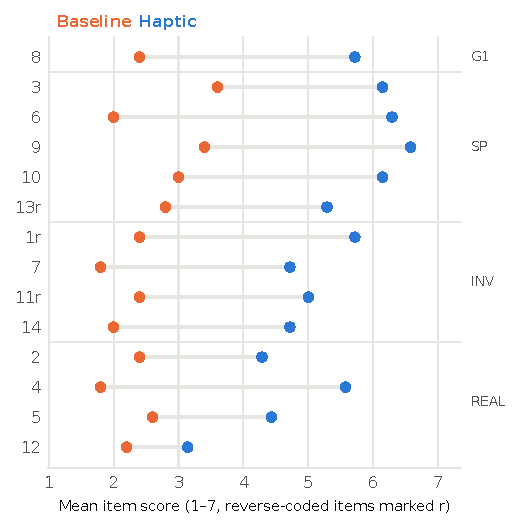
\includegraphics[width=\columnwidth]{figures/ipq_items}
  \caption{Mean score per IPQ item and condition (haptic $n=7$, baseline $n=5$), grouped by subscale; reverse-coded items are marked~r.}
  \Description{Dumbbell chart of the fourteen IPQ items. The haptic mean lies to the right of the baseline mean on every item; the gap is smallest for item 12.}
  \label{fig:ipq-items}
\end{figure}

At the item level (Figure~\ref{fig:ipq-items}), the largest gaps appear on item~6 (``I did not feel present in the virtual space'', $+4.3$ after recoding), item~4 (consistency with real-world experience, $+3.8$), and item~1 (awareness of the real surroundings, $+3.3$)---the items closest to what a haptic proxy manipulates. The smallest gap is on item~12 (``The virtual world seemed more realistic than the real world'', $+0.9$), which stayed low in both conditions; unsurprisingly, touching gummy worms does not make a virtual cabin outrank reality. Baseline scores were strikingly low overall (subscale means between 2.2 and 3.0), which we return to in the discussion.

\todoin{Optional: one short paragraph of behavioral observations---refusals, startle reactions, memorable comments during play.}


% !TeX root = ../paper.tex

\section{Discussion}
\label{sec:discussion}

% !TeX root = ../../paper.tex

\subsection{Interpretation}
\label{sec:discussion-findings}

Taken at face value, the results are a strong endorsement of passive haptics: every participant who played both versions reported more presence with the proxies, on every subscale, and the differences are far larger than what presence manipulations typically produce. The direction is consistent with the classic findings~\cite{Hoffman.1998, Insko.2001} and extends them to deliberately aversive materials---confirming a dreaded touch strengthened the illusion rather than breaking it. That the largest item-level gains sit exactly where a haptic proxy should act (feeling present in the space, consistency with real-world experience, and reduced awareness of the real surroundings) adds internal plausibility: the effect concentrates on the items the manipulation targets, and stays smallest where no proxy could help (a virtual cabin seeming \emph{more} real than reality).

The size of the effect still deserves suspicion rather than celebration. Participants could not be blinded---one condition involves visibly laid-out props and a researcher with a spray bottle---and in a within-subject design this invites demand characteristics: participants may have rated the contrast between conditions rather than each experience on its own. The strikingly low baseline scores point the same way. Subscale means of 2--3 are low for a functioning VR experience, which suggests participants used the questionnaire comparatively, pushing the baseline down after (or in anticipation of) the richer haptic version. A between-subject replication, in which each participant sees only one condition, would separate the genuine haptic effect from this contrast effect; we would expect the difference to shrink, though the concentration of gains on touch-related items gives some confidence it would not vanish.

We also note what the data cannot show. The IPQ measures presence, not fear or disgust, so whether the proxies made the experience \emph{scarier}---our original motivation---remains formally unmeasured. The involvement subscale's gain of $+2.65$ is at least suggestive: participants with proxies reported being far less aware of the room, the researchers, and the sounds around them, which in a horror context is where dread lives.

% !TeX root = ../../paper.tex

\subsection{Limitations}
\label{sec:discussion-limitations}

Several constraints qualify our results. The sample is small: seven participants, of whom five completed both conditions, so the paired analysis rests on five pairs, and the exact Wilcoxon test cannot reach significance at that size. The inferential statistics orient; they prove nothing. We collected no demographic data beyond an observed age range and a gender count. Because the two single-condition participants played the haptic version, the descriptive condition means also draw on different groups. We measured presence with a single questionnaire; without an emotional measure such as the Self-Assessment Manikin or physiological data such as heart rate variability, the emotional side of the question (does the touch make it scarier, beyond making it more present?) rests on anecdote. The IPQ is a blunt instrument for a manipulation aimed at one dimension above all~\cite{presence-questionnaires}.

The within-subject design carries a specific cost in a horror context: a participant who plays the haptic condition second knows the scares by then, and one who plays it first may brace for touches that the baseline never delivers. Counterbalancing distributes this effect across conditions without removing it. The pipe challenge adds a human factor, since a researcher operated the water spray by hand and its timing and intensity varied between sessions. The study procedure was informal in ways a full research project would not permit: participants gave verbal consent with no written forms, and the study room was a regular work room, so ambient noise and the visible presence of the experimenters may have pulled participants out of the experience in ways we could not measure. \todoin{Add anything you noticed during the sessions---tracking hiccups, a proxy that repeatedly misaligned, participants peeking under the headset.}


% !TeX root = ../paper.tex

\section{Conclusion}
\label{sec:conclusion}

% !TeX root = ../../paper.tex

We built a VR horror experience in which every dreadful thing the player must touch is really there to be touched, in proxy form: rubber balls for eyes, gummy worms for worms, a hidden water spray for a burst pipe, synthetic webbing for cobwebs. The technical recipe is deliberately reproducible---consumer hardware, asset-store content, spatial anchors, printed fiducial markers, and props from a supermarket and a Halloween aisle. Our within-subject comparison of the experience with and without these proxies, measured with the IPQ, \todoin{summarize the outcome in one sentence}.

Beyond the specific numbers, the project's practical lesson is that the hard part of passive haptics is not the props but the alignment: the illusion lives or dies on whether the hand meets the object exactly where the eyes expect it, which is a calibration problem more than a design problem. Future work has an obvious next step in restoring the measures we cut---SAM and physiological data such as heart rate variability would separate presence from fright, which the IPQ alone cannot do. A per-challenge manipulation could then identify which kinds of touch (immersion, sudden stimulus, clinging texture) carry the effect, and whether dread needs the hand to be met at all, or only the fear that it might be.


% !TeX root = ../paper.tex

\begin{acks}
  % !TeX root = ../../paper.tex

We thank Prof.\ Dr.\ Jörg Berdux, who supervised this master project, for his support and feedback throughout its development and evaluation. We also thank all participants of the study.

\end{acks}


\bibliographystyle{ACM-Reference-Format}
\bibliography{bibliography}

\end{document}
